\label{fs-framework}

Let us consider the news topic classification as an illustration of a text stream multi-classification task. Input stream contains raw article texts that must be labeled by a classifier and delivered to end-user. The ultimate purpose is to achieve the distribution of news topics that is changing over time. This task is a typical representative of the text stream classification problem.

A widespread classification pipeline used in batch processing systems~\cite{semberecki2016distributed} is based on bag-of-words text representation and consists of two steps. The first one is computing TF-IDF features. The second one is training a classifier on these features or making a prediction. Such pipelines are commonly represented it in the form of a {\em logical execution graph}. It serves as a language for defining pipelined computations in the majority of popular batch and stream processing systems~\cite{Carbone:2017:SMA:3137765.3137777, Zaharia:2016:ASU:3013530.2934664, apache:storm, Kulkarni:2015:THS:2723372.2742788, Noghabi:2017:SSS:3137765.3137770}. Vertices of the logical graph denote operations, while edges indicate data subscriptions between them. 

The starting point in a text classification data flow is a {\em Source} vertex. It receives input texts from data producers and computes term frequencies. Computation of inverse document frequencies is a separate operation because it maintains a state and requires different data partitioning in a physical execution. {\em TF-IDF} vertex joins features corresponding to the same text and passes them to the {\em Text Classifier}. {\em Text Classifier} is the very last vertex that predicts a labels distribution for the document and delivers it to a data consumer. The scheme of the proposed logical graph is shown in Figure~\ref{logical_graph}. It is important to note that this data flow only provides for prediction. 
We show how to incorporate training into this graph  in section~\ref{fs-solution}.


\begin{figure}[htbp]
  \centering
  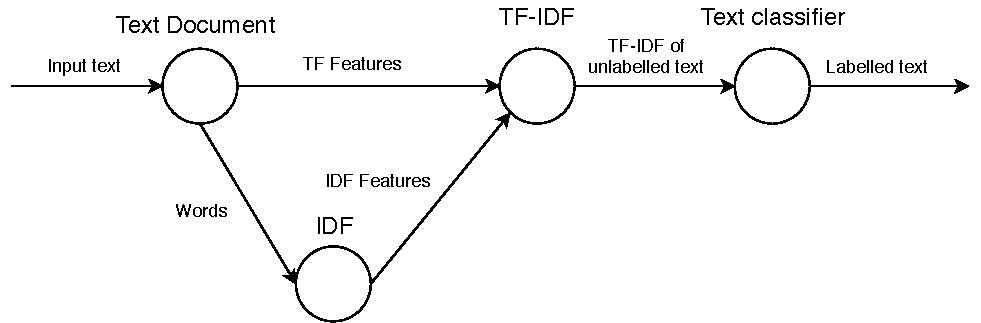
\includegraphics[scale=0.52]{pics/logical-graph-no-part-fit}
  \caption{Logical graph for text classification}
  \label {logical_graph}
\end{figure}

Typical execution of this logical graph is illustrated in Figure~\ref{physical_graph}. Each vertex on the scheme denotes the same computational cluster consisted of multiple units. The data partition is defined by a key, which is a word for {\em IDF} operation and document identifier for {\em TF-IDF} aggregator. Data elements with the same keys are processed on a single computational unit.

\begin{figure}[htbp]
  \centering
  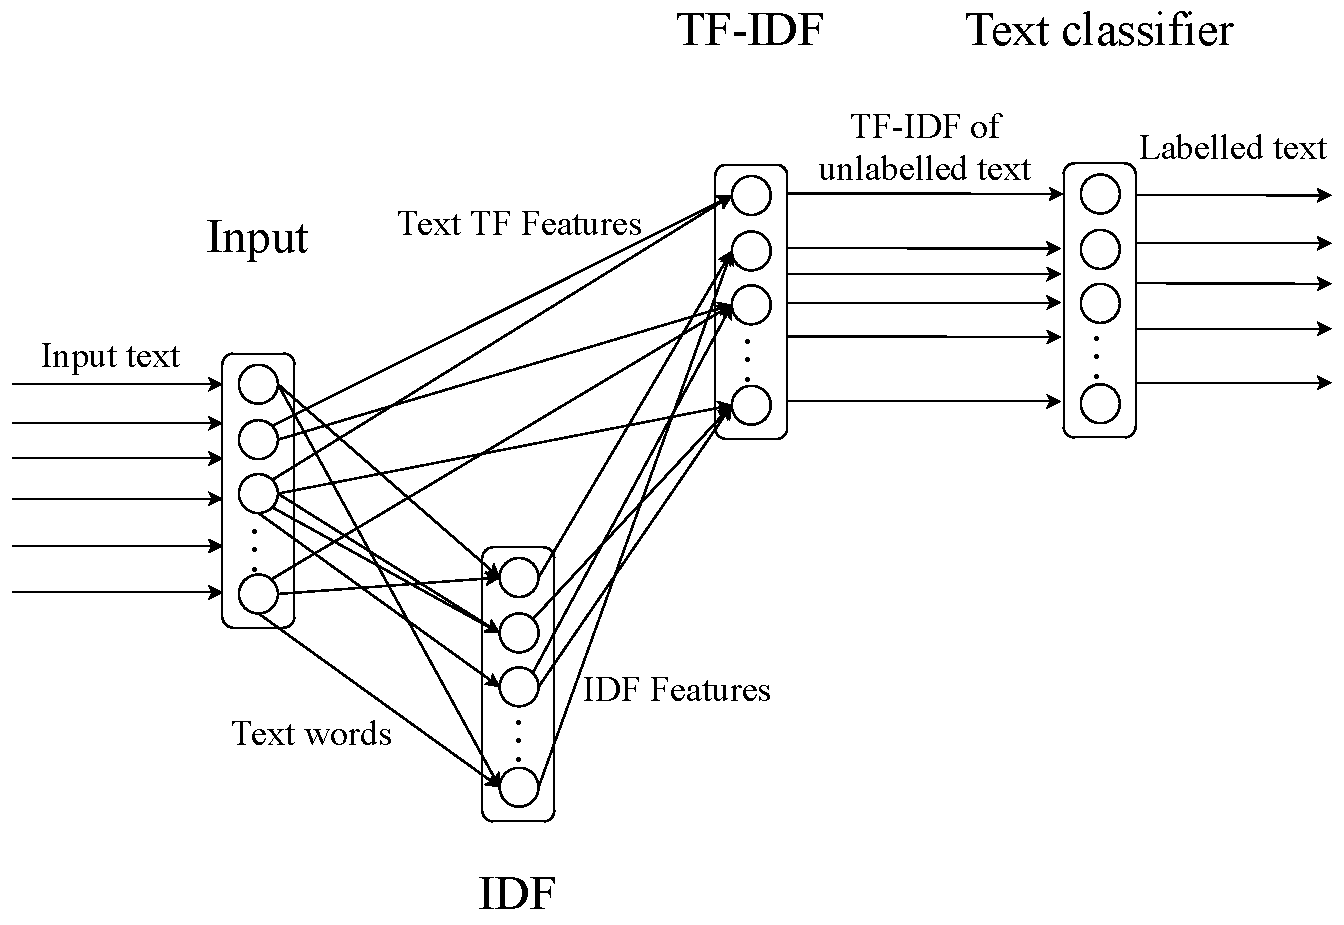
\includegraphics[scale=0.375]{pics/physical-graph-no-part-fit}
  \caption{Physical graph for text classification}
  \label {physical_graph}
\end{figure}

Despite the fact that the proposed data flow is commonly used for batch processing systems~\cite{semberecki2016distributed}, it has several potential issues regarding its execution on top of distributed stream processing engine:

\begin{itemize}
    \item There can be a race between elements before the update of {\em IDF} due to multiple asynchronous network channels as it is shown in Figure~\ref{physical_graph}. 
     sorting data before an operation is natural for batch processing systems,     It  is not appropriate in stream processing systems      due to strong low latency requirements.
    It is  not    clear how such reorderings during the physical execution influence classification results.
    
    \item 
    In contrast with batch processing systems, streaming engines usually do not provide the same level of fault tolerance, e.g. within at least once guarantee, some input texts may be processed multiple times. Such behavior can potentially cause biased results. On the other hand, existing approaches to achieve exactly once provide high performance overhead~\cite{we2018beyondmr} that can be unacceptable for applications which require extremely low latency.
\end{itemize}